\secA{Outputs}
\label{sec-output}

\secB{During execution}

\duchamp\ provides the user with feedback whilst it is running, to
keep the user informed on the progress of the analysis. Most of this
consists of self-explanatory messages about the particular stage the
program is up to. The relevant parameters are printed to the screen at
the start (once the file has been successfully read in), so the user
is able to make a quick check that the setup is correct (see
Appendix~{app-input} for an example).

If the cube is being trimmed (\S\ref{sec-modify}), the resulting
dimensions are printed to indicate how much has been trimmed. If a
reconstruction is being done, a continually updating message shows
either the current iteration and scale, compared to the maximum scale
(when \texttt{reconDim=3}), or a progress bar showing the amount of
the cube that has been reconstructed (for smaller values of
\texttt{reconDim}).

During the searching algorithms, the progress through the 1D and 2D
searches are shown. When the searches have completed, the number of
objects found in both the 1D and 2D searches are reported (see
\S\ref{sec-detection} for details).

In the merging process (where multiple detections of the same object
are combined -- see \S\ref{sec-merger}), two stages of output
occur. The first is when each object in the list is compared with all
others. The output shows two numbers: the first being how far through
the list the current object is, and the second being the length of the
list. As the algorithm proceeds, the first number should increase and
the second should decrease (as objects are combined). When the numbers
meet (\ie the whole list has been compared), the second phase begins,
in which multiply-appearing pixels in each object are removed, as are
objects not meeting the minimum channels requirement. During this
phase, the total number of accepted objects is shown, which should
steadily increase until all have been accepted or rejected. Note that
these steps can be very quick for small numbers of detections.

Since this continual printing to screen has some overhead of time and
CPU involved, the user can elect to not print this information by
setting the parameter \texttt{verbose = 0}. In this case, the user is
still informed as to the steps being undertaken, but the details of
the progress are not shown.

\secB{Results}

\secC{Table of results}

Finally, we get to the results -- the reason for running \duchamp\ in
the first place. Once the detection list is finalised, it is sorted by
the mean velocity of the detections (or, if there is no good WCS
associated with the cube, by the mean Z-pixel position). The results
are then printed to the screen and to the output file, given by the
\texttt{OutFile} parameter. The results list, an example of which can
be seen in Appendix~\ref{app-output}, contains the following columns
(note that the title of the columns depending on WCS information will
depend on the projection of the WCS):

\begin{entry}
\item[Obj\#] The ID number of the detection (simply the sequential
  count for the list, which is ordered by increasing velocity, or
  channel number, if the WCS is not good enough to find the velocity).
\item[Name] The ``IAU''-format name of the detection (derived from the
  WCS position -- see below for a description of the format).
\item[X] The average X-pixel position (averaged over all detected
voxels).
\item[Y] The average Y-pixel position.
\item[Z] The average Z-pixel position.
\item[RA/GLON] The Right Ascension or Galactic Longitude of the centre
of the object.
\item[DEC/GLAT] The Declination or Galactic Latitude of the centre of
the object.
\item[VEL] The mean velocity of the object [units given by the
  \texttt{spectralUnits} parameter].
\item[w\_RA/w\_GLON] The width of the object in Right Ascension or
Galactic Longitude [arcmin].
\item[w\_DEC/w\_GLAT] The width of the object in Declination Galactic
  Latitude [arcmin].
\item[w\_VEL] The full velocity width of the detection (max channel
  $-$ min channel, in velocity units [see note below]).
\item[F\_int] The integrated flux over the object, in the units of
  flux times velocity, corrected for the beam if necessary.
\item[F\_peak] The peak flux over the object, in the units of flux.
\item[X1, X2] The minimum and maximum X-pixel coordinates.
\item[Y1, Y2] The minimum and maximum Y-pixel coordinates.
\item[Z1, Z2] The minimum and maximum Z-pixel coordinates.
\item[Npix] The number of voxels (\ie distinct $(x,y,z)$ coordinates)
  in the detection.
\item[Flag] Whether the detection has any warning flags (see below).
\end{entry}
The Name is derived from the WCS position. For instance, a source
centred on the RA,Dec position 12$^h$53$^m$45$^s$,
-36$^\circ$24$'$12$''$ will be called J125345$-$362412 (if the epoch
is J2000) or B125345$-$362412 (if B1950). An alternative form is used
for Galactic coordinates: a source centred on the position ($l$,$b$) =
(323.1245, 5.4567) will be called G323.124$+$05.457. If the WCS is not
valid (\ie is not present or does not have all the necessary
information), the Name, RA, DEC, VEL and related columns are not
printed, but the pixel coordinates are still provided.

The velocity units can be specified by the user, using the parameter
\texttt{spectralUnits} (enter it as a single string). The default
value is km/s, which should be suitable for most users. These units
are also used to give the units of integrated flux. Note that if there
is no rest frequency specified in the FITS header, the \duchamp\
output will instead default to using Frequency, with units of MHz.

If the WCS is not specified sufficiently to be used, then all columns
from RA/GLON to w\_VEL will be left blank. Also, F\_int will be
replaced with the more simple F\_tot -- the total flux in the
detection, being the sum of all detected voxels.

The last column contains any warning flags about the detection. There
are currently two options here. An `E' is printed if the detection is
next to the edge of the image, meaning either the limit of the pixels,
or the limit of the non-BLANK pixel region. An `N' is printed if the
total flux, summed over all the (non-BLANK) pixels in the smallest box
that completely encloses the detection, is negative. Note that this
sum is likely to include non-detected pixels. It is of use in pointing
out detections that lie next to strongly negative pixels, such as
might arise due to interference -- the detected pixels might then also
be due to the interference, so caution is advised.

\secC{Other results lists}

Two alternative results files can also be requested. One option is a
VOTable-format XML file, containing just the RA, Dec, Velocity and the
corresponding widths of the detections, as well as the fluxes. The
user should set \texttt{flagVOT = 1}, and put the desired filename in
the parameter \texttt{votFile} -- note that the default is for it not
to be produced. This file should be compatible with all Virtual
Observatory tools (such as Aladin\footnote{ Aladin can be found on the
web at
\href{http://aladin.u-strasbg.fr/}{http://aladin.u-strasbg.fr/}}). The
second option is an annotation file for use with the Karma toolkit of
visualisation tools (in particular, with \texttt{kvis}). This will
draw a circle at the position of each detection, and number it
according to the Obj\# given above. To make use of this option, the
user should set \texttt{flagKarma = 1}, and put the desired filename
in the parameter \texttt{karmaFile} -- again, the default is for it
not to be produced.

As the program is running, it also (optionally) records the detections
made in each individual spectrum or channel (see \S\ref{sec-detection}
for details on this process). This is recorded in the file given by
the parameter \texttt{LogFile}. This file does not include the columns
\texttt{Name, RA, DEC, w\_RA, w\_DEC, VEL, w\_VEL}. This file is
designed primarily for diagnostic purposes: \eg to see if a given set
of pixels is detected in, say, one channel image, but does not survive
the merging process. The list of pixels (and their fluxes) in the
final detection list are also printed to this file, again for
diagnostic purposes. The file also records the execution time, as well
as the command-line statement used to run \duchamp. The creation of
this log file can be prevented by setting \texttt{flagLog =
false}. (This may be a good idea if you are not interested in its
contents, as it can be a large file if many pixels are being
detected.)

\secC{Graphical output -- spectra}

\begin{figure}[t]
\begin{center}
\includegraphics[width=\textwidth]{example_spectrum}
\end{center}
\caption{\footnotesize An example of the spectrum output. Note several
  of the features discussed in the text: the red lines indicating the
  reconstructed spectrum; the blue dashed lines indicating the
  spectral extent of the detection; the green hashed area indicating
  the Milky Way channels that are ignored by the searching algorithm;
  the blue border showing its spatial extent on the 0th moment map;
  and the 15~arcmin-long scale bar.}
\label{fig-spect}
\end{figure}

\begin{figure}[!t]
\begin{center}
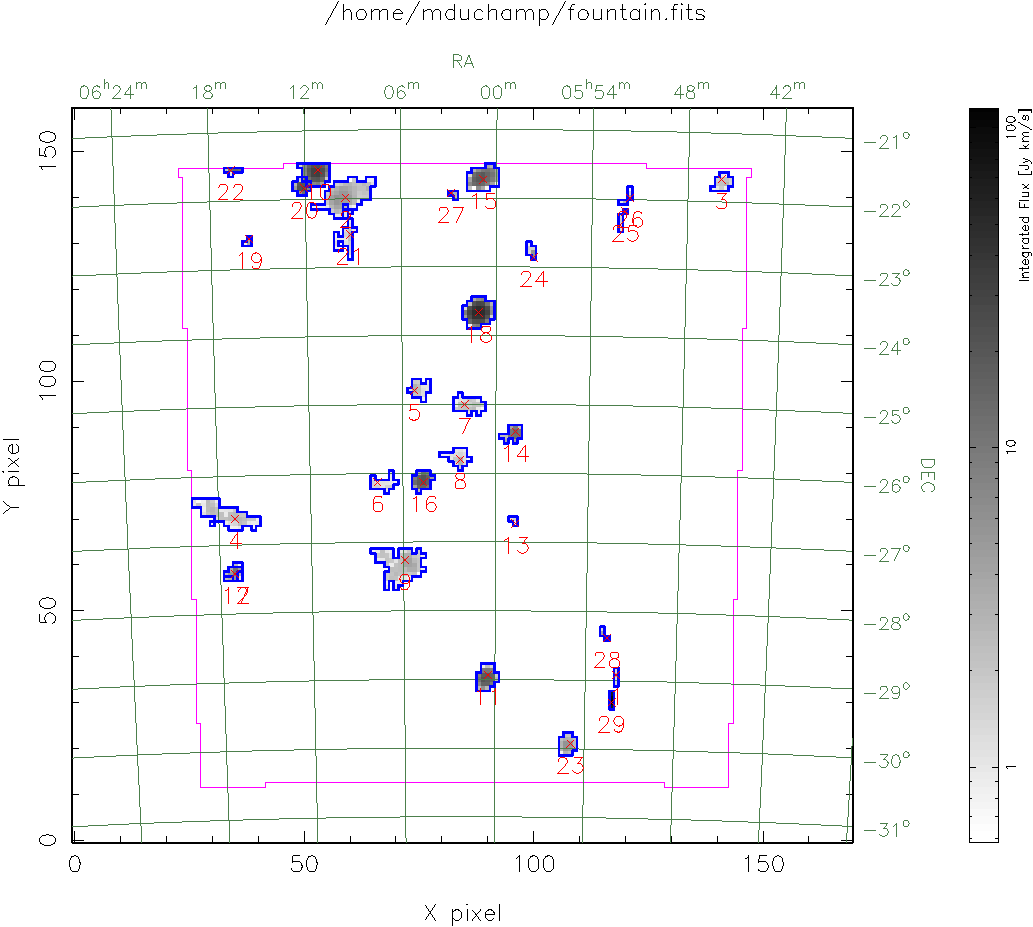
\includegraphics[width=\textwidth]{example_moment_map}
\end{center}
\caption{\footnotesize An example of the moment map created by
  \duchamp. The full extent of the cube is covered, and the 0th moment
  of each object is shown (integrated individually over all the
  detected channels). The purple line indicates the limit of the
  non-BLANK pixels.}
\label{fig-moment}
\end{figure}

As well as the output data file, a postscript file is created that
shows the spectrum for each detection, together with a small cutout
image (the 0th moment) and basic information about the detection (note
that any flags are printed after the name of the detection, in the
format \texttt{[E]}). If the cube was reconstructed, the spectrum from
the reconstruction is shown in red, over the top of the original
spectrum. The spectral extent of the detected object is indicated by
two dashed blue lines, and the region covered by the ``Milky Way''
channels is shown by a green hashed box. An example detection can be
seen below in Fig.~\ref{fig-spect}.

The spectrum that is plotted is governed by the
\texttt{spectralMethod} parameter. It can be either \texttt{peak},
where the spectrum is from the spatial pixel containing the
detection's peak flux; or \texttt{sum}, where the spectrum is summed
over all spatial pixels, and then corrected for the beam size.  The
spectral extent of the detection is indicated with blue lines, and a
zoom is shown in a separate window.

The cutout image can optionally include a border around the spatial
pixels that are in the detection (turned on and off by the parameter
\texttt{drawBorders} -- the default is \texttt{true}). It includes a
scale bar in the bottom left corner to indicate size -- its length is
indicated next to it (the choice of length depends on the size of the
image).

There may also be one or two extra lines on the image. A yellow line
shows the limits of the cube -- the detected object is obviously close
to the edge of the cube, and the box size extends outside the region
covered by the data. A purple line, however, shows the dividing line
between BLANK and non-BLANK pixels. The BLANK pixels will always be
shown in black. The first type of line is always drawn, while the
second is governed by the parameter \texttt{drawBlankEdges} (whose
default is \texttt{true}), and obviously whether there are any BLANK
pixel present.

\secC{Graphical output -- maps}

Finally, a couple of images are optionally produced: a 0th moment map
of the cube, combining just the detected channels in each object,
showing the integrated flux in grey-scale; and a ``detection image'',
a grey-scale image where the pixel values are the number of channels
that spatial pixel is detected in. In both cases, if
\texttt{drawBorders = true}, a border is drawn around the spatial
extent of each detection, and if \texttt{drawBlankEdges = true}, the
purple line dividing BLANK and non-BLANK pixels (as described above)
is drawn. An example moment map is shown in Fig.~\ref{fig-moment}.
The production or otherwise of these images is governed by the
\texttt{flagMaps} parameter.

The purpose of these images are to provide a visual guide to where the
detections have been made, and, particularly in the case of the moment
map, to provide an indication of the strength of the source. In both
cases, the detections are numbered (in the same sense as the output
list and as the spectral plots), and the spatial borders are marked
out as for the cutout images in the spectra file. Both these images
are saved as postscript files (given by the parameters
\texttt{momentMap} and \texttt{detectionMap} respectively), with the
latter also displayed in a \textsc{pgplot} window (regardless of the
state of \texttt{flagMaps}).
